\documentclass[11pt,a4paper]{report}
\usepackage[utf8]{inputenc}
\usepackage[french]{babel}
\usepackage[T1]{fontenc}
\usepackage{amsmath}
\usepackage{amsfonts}
\usepackage{amssymb}
\usepackage{xcolor}
\usepackage{gensymb}

\usepackage{geometry}
\geometry{hmargin=2.5cm,vmargin=1.5cm}
\usepackage{wasysym}
\usepackage{graphicx}

\author{Mathieu Sarrat}
\title{LP7 - Transitions de phase}

\makeatletter
\renewcommand{\thesection}{\@arabic\c@section}
\makeatother


\begin{document}
\maketitle

\section*{Pré-requis, matériel, recommandations}

\subsubsection*{Niveau : Licence de physique}

\subsubsection*{Pré-requis :}
\begin{itemize}
	\item Premier et Second Principe de la Thermodynamique.
	\item Potentiels thermodynamiques.
	\item Notions sur les milieux magnétiques : paramagnétisme et ferromagnétisme.
\end{itemize}

\subsubsection*{Matériel :}
\begin{itemize}
	\item Vase Dewar
	\item Résistance chauffante et alimentation (compter 400 W)
	\item Thermomètre à résistance de platine (Pt100)
	\item Balance (pouvant supporter une charge de plusieurs kilos)
	\item Potence en bois
	\item Sèche-cheveux
\end{itemize}

\section*{Introduction}

Les transitions de phase sont des phénomènes qui correspondent de façon générale à un \textbf{changement qualitatif et quantitatif des propriétés macroscopiques} de la matière lorsqu'on fait varier un paramètre de contrôle du système. Ils se produisent lorsqu'une phase thermodynamique devient instable dans des conditions extérieures données.

\newpage
\section{Changement d'état du corps pur}

Un corps pur peut, suivant les conditions qui lui sont imposées, se présenter sous diverses phases : liquide, solide, gaz. On se propose d'analyser le \textbf{passage d'une phase à l'autre, appelé changement d'état} et les conditions de coexistence à l'équilibre de plusieurs phases d'un même corps pur.\\

Dans notre vie quotidienne, observe régulièrement l'eau sous ses trois phases principales : on rencontre le plus souvent de l'eau liquide (sa phase liquide), mais aussi la glace (phase solide) et la vapeur d'eau (sa phase gazeuse). On parle de \textbf{vaporisation} lorsqu'on transforme le liquide en gaz, de \textbf{fusion} lorsque le solide fond en liquide et de sublimation lorsqu'on transforme le solide en gaz. Les transformations inverses sont respectivement la condensation, la solidification et la condensation solide.\\

\begin{figure}[h!]
	\begin{center}
		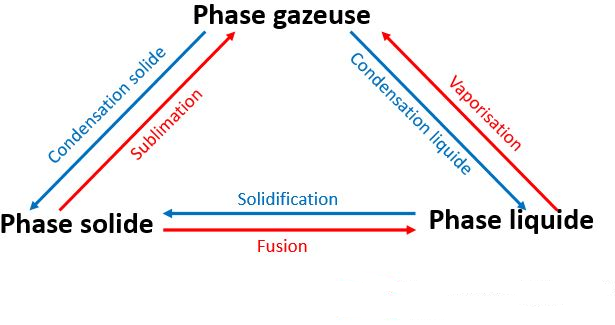
\includegraphics[scale = 0.45]{changement_etat.png}
	\end{center}
	\caption{Changements d'état de la matière.}
\end{figure}

Tous les corps purs, pas seulement l'eau, subissent des changements d'état, dans des conditions plus ou moins facilement réalisables en pratique. Sous pression atmosphérique, le mercure se solidifie à 234.3 K (soit -38.9 \degree C) et se vaporise à 629.8 K (soit 356.6 \degree C). Le diazote, constituant majoritaire de l'atmosphère terrestre, gèle à 63.14 K et bout à 77.36 K. La fusion des métaux par chauffage est réalisée depuis des siècles, dans les forges et les fonderies.

\subsection{Transition liquide-vapeur}

Nous allons maintenant nous appuyer sur le cas de la transition liquide-vapeur pour dégager plusieurs résultats généraux concernant le changement d'état d'un corps pur.

\subsubsection*{Évolution à température constante}

Soit $n$ moles de corps pur à l'état gazeux enfermées dans un récipient diatherme dont une des parois est un piston mobile. On fait subir à ce corps une transformation isotherme : pour cela, on suppose le récipient en contact avec un thermostat qui maintient une température uniforme et stationnaire $T$ dans le système, et on comprime de façon réversible

 le gaz de sorte que sa pression soit constamment définie durant la transformation.\\

\begin{figure}[h!]
	\begin{center}
		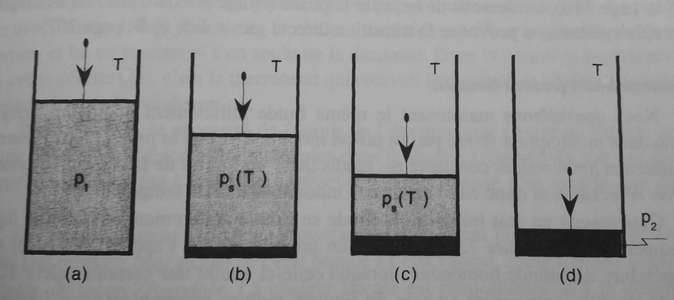
\includegraphics[scale = 0.45]{transfo_tcte.png}
	\end{center}
	\caption{Transformation à température constante.}
\end{figure}

Deux cas sont observés, selon que la température du thermostat est supérieure ou non à une \textbf{température critique} $T_c$ :
\begin{itemize}
	\item 1\degree) $T \leq T_c$ : au début de la transformation, la pression augmente au fur et à 			mesure qu'on comprime le gaz. Apparait ensuite une goutte de liquide au fond du piston : la 		pression à une valeur $p_s$. Au fur et à mesure qu'on comprime, la quantité de liquide 				augmente alors que celle de gaz diminue. La pression reste stable, égale à $p_s$ tant qu'il 		reste du gaz dans l'enceinte. La valeur $p_s$ de ce \textbf{palier de pression}, qu'on 				appelle \textbf{pression de vapeur saturante}, est une fonction croissante de la 					température. Le gaz disparu, la pression augmente à nouveau si on continue à comprimer.\\ 
	\item 2\degree) $T > T_c$, le fluide reste homogène quelque soit le volume de l'enceinte, on 			n'observe pas de changement d'état. Nous verrons plus loin que nous sommes dans un régime 			où la distinction entre liquide et gaz n'a plus de sens. On préfèrera parler de fluide 				supercritique.
\end{itemize}
 
\subsubsection*{Évolution à pression constante}

On part initialement d'une quantité $n$ d'eau liquide contenue dans le même récipient et on fait le choix de travailler à pression constante, par exemple à pression atmosphérique $p_0$. Le système est à l'équilibre avec ce barostat et $p = p_0$ est constante et homogène dans tout le liquide. Admettons qu'on fournisse de la chaleur de façon réversible au système de sorte que la température soit constamment définie au cours de la transformation. Qu'observera-t-on ?\\

Là aussi, une pression limite se manifeste, qu'on appelle \textbf{pression critique} : on n'observe pas de transition liquide-vapeur si $p > p_c$ et la température augmente au fur et à mesure de l'apport de chaleur.\\

\begin{figure}[h!]
	\begin{center}
		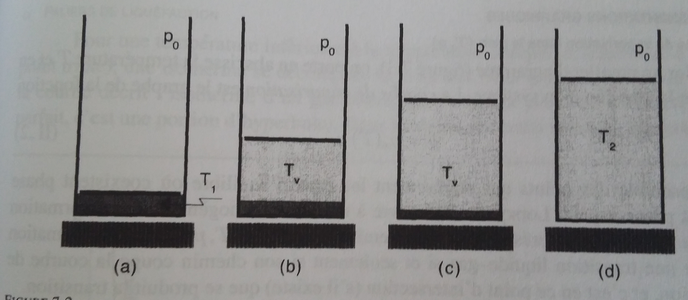
\includegraphics[scale = 0.45]{transfo_pcte.png}
	\end{center}
	\caption{Transformation à température constante.}
\end{figure}

Si $p < p_c$, l'apport de chaleur commence par élever la température du liquide jusqu'à une température $T_\text{vap}$ à laquelle apparaît la phase gazeuse. On continue de chauffer, et on constate quelque chose de contre-intuitif : la température reste constante tant que liquide et gaz coexistent. Ce n'est que lorsque la dernière goutte de liquide disparaît que la température recommence à croître. On a donc un \textbf{palier de température} lorsque les deux phases coexistent et $T_\text{vap}$ est appelée \textbf{température de vaporisation} (de façon générale, on parle de température de changement d'état, car ce palier est présent quelque soit le changement d'état à pression constante réalisé, notamment solide-liquide).\\

\begin{figure}
	\begin{center}
		\begin{tabular}{|c|c|c|}
			\hline
			Corps pur & $T_\text{fus}$ (K) & $T_\text{vap}$ (K) \\
			\hline
			Eau & 273.15 & 373.15\\
			\hline
			Mercure & 234 & 630\\
			\hline
			Diazote & 63 & 77.4\\
			\hline
			Étain & 505 & 2543\\
			\hline
			Titane & 1941 & 6203\\
			\hline
		\end{tabular}
	\end{center}
	\caption{Quelques valeurs de températures de changement d'état sous pression normale 
	$p = 101 325$ Pa.}
\end{figure}

\subsection{Chaleur latente}

Coupons l'afflux de chaleur lors de la transformation précédente : les quantités de vapeur et de liquide présentes dans le récipient restent constantes, à l'équilibre l'une avec l'autre. La chaleur fournie permet de produire de la vapeur. En soustraire réduit la quantité de vapeur et augmente celle de liquide. Dans les deux cas, la température ne varie pas. Ce besoin de fournir de l'énergie pour passer du liquide au gaz résulte d'une cohésion plus forte de la matière à l'état liquide qu'à l'état gazeux.\\

On appelle \textbf{chaleur latente de vaporisation} la quantité de chaleur $\mathcal{L}_\text{vap}$ qu'il faut fournir à une quantité d'eau liquide pour la transformer intégralement en vapeur, \textbf{à température et pression constante et ce de façon réversible}.\\

On va maintenant mesurer la chaleur latente de vaporisation de l'eau. La chaleur fournie à l'eau est contrôlée par une résistance chauffante de puissance $P_J$ immergée dans l'eau contenue dans un vase Dewar. Lorsque l'eau bout, on mesure la masse d'eau vaporisée $\Delta m = m(t) - m(0)$ au cours du temps, grâce à une balance. La chaleur fournie à l'eau en ébullition pendant la durée $\Delta t$ de l'expérience est utilisée pour réaliser le changement d'état, d'où
\begin{equation}
	P_J \Delta t = \Delta m \;\mathcal{L}_\text{vap},
\end{equation}
d'où
\begin{equation}
	\boxed{m(t) = m(0) + \frac{P_J}{\mathcal{L}_\text{vap}}t}.
\end{equation}

\textcolor{red}{Manip : vaporisation de l'eau contenue dans un Dewar contenant une résistance chauffante}

\begin{itemize}
	\item Connecter la résistance chauffante à un générateur adapté, muni d'un wattmètre. Plonger 			dans un Dewar contenant de l'eau. Régler le générateur pour que la résistance fournisse 			entre 400 à 500 W et noter la valeur.
	\item Utiliser une potence légère ou utiliser une balance pouvant encaisser suffisamment de 			masse. Poser la potence sur la balance permet de s'affranchir de la poussée d'Archimède.
	\item Atteindre l'ébullition \textbf{avant} le début de la leçon pour ne pas perdre de temps.
	\item Placer et allumer un sèche-cheveux au-dessus du Dewar : on chasse la vapeur d'eau générée 		par l'ébullition, ce qui limite le risque qu'elle se recondense, et donc de chauffer deux 			fois la même quantité d'eau.
	\item Mesurer la température pendant l'ébullition.
	\item Tarer la balance au moment de commencer les mesures, relever toutes les 10 secondes la 			masse d'eau qui s'est évaporée pendant 2 minutes. Reporter les valeurs de masse et de temps 		sur Regressi, assorties de leur incertitude. 
	\item Vérifier le caractère linéaire de l'évolution, utiliser la pente et la mesure de $P_J$ 			pour remonter à $\mathcal{L}_\text{vap}$.\\ 
\end{itemize}

\begin{figure}
	\begin{center}
		\begin{tabular}{|c|c|c|c|}
			\hline
			Corps pur & $\mathcal{L}_\text{fus}$ (kJ/mol) 
				& $\mathcal{L}_\text{vap}$ (kJ/mol) & Masse molaire (g/mol)\\
			\hline
			Eau & 6 & 40.7 & 18.015\\
			\hline
			Mercure & 2.3 & 58.1 & 200.6\\
			\hline
			Diazote & 0.7 & 5.6 & 28.013\\
			\hline
			Étain & 7.1 & 290.4 & 118.7\\
			\hline
			Titane & 15.5 & 429 & 47.867\\
			\hline
		\end{tabular}
	\end{center}
	\label{tab:chaleurlat}
	\caption{Chaleurs latentes de fusion et de vaporisation sous p $= 101325$ Pa.}
\end{figure}

Les chaleurs latentes sont des énergies énormes comme on peut le voir dans le tableau \ref{tab:chaleurlat}. Les changements d'état consomment donc beaucoup d'énergie. Ce n'est pas étonnant si le corps humain se sert de ce phénomène pour se refroidir lorsqu'il fait chaud : en s'évaporant, la sueur refroidit l'organisme (on prélève de la chaleur dans le corps pour vaporiser l'eau).

\subsection{Représentations graphiques}

On utilise des diagrammes pour représenter l'état du corps pur en fonction des conditions de température, de pression et de volume.

\subsubsection*{Diagramme de phases}

On va donc tracer dans l'espace $(T,p)$ la courbe $p_s(T)$ décrivant l'ensemble des états où liquide et vapeur coexistent à l'équilibre, c'est à dire les états pour lesquels le corps pur est présent sous deux phases stables : c'est la \textbf{courbe de vaporisation}. Si on fait suivre au corps pur une transformation réversible quelconque, représentée par un chemin dans le plan $(T,p)$, qui traverse la courbe de vaporisation, cela signifie que le corps pur va subir une transition de phase liquide-vapeur. C'est au point d'intersection entre cette trajectoire et la courbe de vaporisation qu'à lieu la transition de phase : les coordonnées de ce point nous renseignent sur la pression et la température à laquelle aura lieu la transition. On représente de même les courbes de fusion (resp. de sublimation), décrivant les états pour lesquels les phases solide et liquide (resp. solide et vapeur) coexistent à l'équilibre.

\begin{figure}[h!]
	\begin{center}
		\begin{tabular}{cc}
			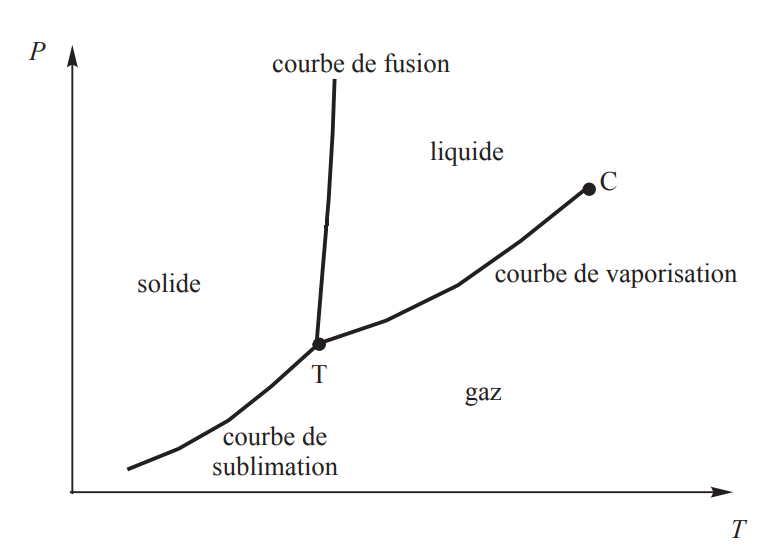
\includegraphics[scale = 0.35]{pT_standard.png}&
			\includegraphics[scale = 0.35]{pT_BiAgH2O.png}\\
		\end{tabular}
	\end{center}
	\caption{Diagramme de phases $(T,p)$ : à gauche, le cas le plus courant pour lequel la courbe de fusion a une pente positive. \`A droite le cas correspondant à l'eau, à l'argent et au bismuth 	(parmi d'autres corps purs) : la pente est décroissante.}
\end{figure}

Ces courbes délimitent chacune deux domaines distincts : par exemple le domaine de stabilité du liquide et celui de la vapeur pour la courbe de vaporisation. On doit souligner la présence de deux points notables :
\begin{itemize}
	\item d'une part le \textbf{point triple} ($T_T,p_T$) en lequel les phases solides, liquide et vapeur coexistent à l'équilibre;
	\item d'autre part le \textbf{point critique} ($T_c,p_c,$) au-delà duquel ($T > T_c$ \textbf{et} $p > p_c$) il est \textbf{impossible de distinguer les phases liquide et vapeur}, on parle de fluide supercritique. Lors d'une compression isotherme à $T > T_c$ il est impossible de distinguer deux phases, il n'y a donc pas de transition de phase. Il est ainsi possible de passer de l'état liquide à l'état gazeux sans transition de phase, en \textbf{contournant le point critique}. 
\end{itemize}
 
On remarquera que les courbes de sublimation et de fusion ne présentent pas de point critique, ce que l'on peut comprendre en considérant la structure microscopique d'un solide : ordonnée et donc fondamentalement différente de celle d'un liquide ou d'un gaz. Microscopiquement, il n'y a pas de différence fondamentale entre un liquide et un gaz, ce qui nous permet de les distinguer est la distance moyenne entre les particules, et donc l'intensité des interactions qui les lient.

\begin{figure}
	\begin{center}
		\begin{tabular}{|c|c|c|c|c|}
			\hline
			Corps pur & $T_T$ (K) & $p_T$ (Pa) & $T_c$ (K) & $p_C$ (atm)\\
			\hline
			Eau & 273.16 & 611 & 647.4 & 218.3 \\
			\hline
			Dioxygène & 54.36 & 150 & 154.4 & 49.7\\
			\hline
			Diazote & 63.15 & 12500 & 126.19 & 33.5\\
			\hline
		\end{tabular}
	\end{center}
	\label{tab:tricrit}
	\caption{Points triples et critiques. Rappel : 1 atm $=$ 101325 Pa}
\end{figure} 
 
Un même corps pur à l'état solide peut présenter des structures microscopiques radicalement différentes : on parle de \textbf{variétés allotropiques}. C'est par exemple le cas du fer, avec ses formes $\alpha$ (si $T < T_r$ 1179 K à pression atmosphérique, le réseau est cubique centré) et $\gamma$ (réseau cubique à faces centrées, si $T > T_r$), ou celui de l'eau bien plus complexe (les variétés allotropiques de la glace sont nombreuses). Les transitions de phase entre deux variétés allotropiques sont du premier ordre et sont qualifiées de \textbf{transitions de polymorphisme}.

\begin{figure}[h!]
	\begin{center}
		\begin{tabular}{cc}
			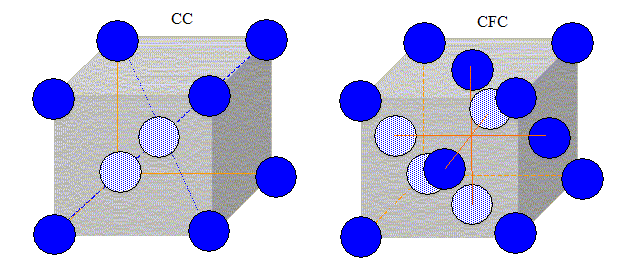
\includegraphics[scale = 0.45]{fer_alpha_gamma.png}&
			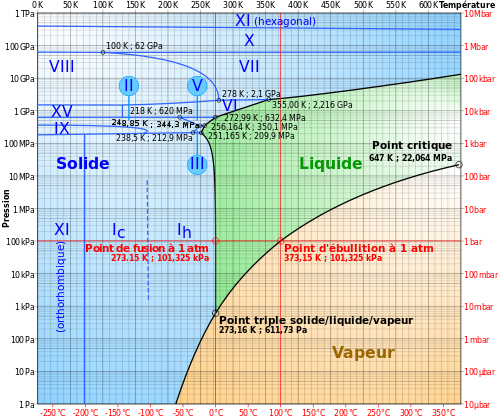
\includegraphics[scale = 0.55]{allotropic.png}\\
		\end{tabular}
	\end{center}
	\caption{\`A gauche : variétés allotropiques du fer, le fer $\alpha$ et le fer $\gamma$. \`A droite : variétés allotropiques de la glace. La glace "habituelle" est la $\text{I}_\text{h}$..}
\end{figure}

\subsubsection*{Diagramme de Clapeyron}

Pour une quantité de matière donnée de corps pur, un point situé dans un domaine
monophasé décrit un unique état caractérisé par $(p,V,T)$ : l'équation d'état du corps pur dans la phase considérée donne le volume V à partir de la pression et de la température.
Par contre, un point situé sur une courbe d'équilibre diphasé décrit une infinité d'états, ayant en commun de mêmes valeurs pour $p$ et $T$ mais des quantités de matière et des volumes différents pour chacune des phases. On utilise donc, en complément du diagramme de phases, d'autres représentations. Nous allons introduire le diagramme $(p,V)$ également appelé diagramme de Clapeyron. On peut tracer dans ce diagramme les courbes représentant les transformations isothermes décrites précédemment : ce sont les \textbf{isothermes d'Andrews}.

\begin{figure}[h!]
	\begin{center}
		\begin{tabular}{cc}
			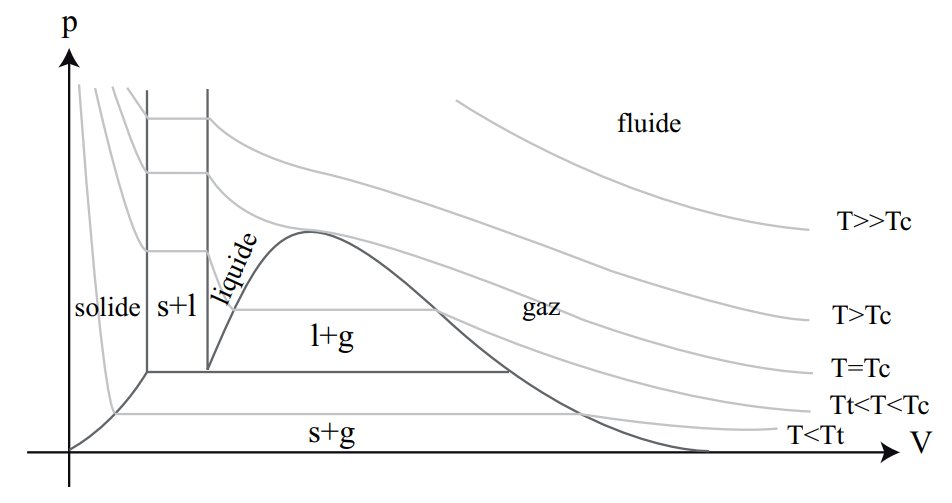
\includegraphics[scale = 0.35]{clapeyron.png}&
			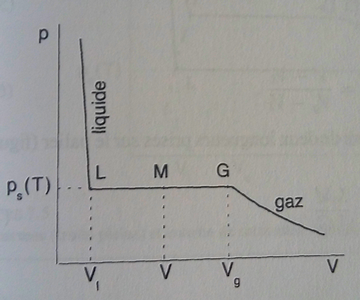
\includegraphics[scale = 0.55]{clapeyronlv.png}\\
		\end{tabular}
	\end{center}
	\caption{\`A gauche : diagramme de Clapeyron complet, sur lequel figure les isothermes 				d'Andrews. \`A droite : diagramme de Clapeyron réduit à la transition liquide-vapeur.}
\end{figure}

Pour une température inférieure à la température critique et supérieure à celle du point triple, une isotherme se décompose en trois morceaux. Pour V grand, l'isotherme est celle d'un gaz homogène. Pour V petit, l'isotherme est celle d'un liquide homogène. Dans les deux cas, la pression décroit avec l'augmentation du volume. Les \textbf{liquides étant faiblement compressibles} ($\chi_T$ petit), la pente de l'isotherme du liquide pur est bien plus forte :
\begin{equation}
	\left(\frac{\partial p}{\partial V}\right)_T = -\frac{1}{V\chi_T}
\end{equation}
où $\chi_T$ est le coefficient de compressibilité isotherme.\\ 

Ces deux arcs sont reliés par un palier horizontal dit \textbf{palier de liquéfaction}, correspondant à la transition de phase : équilibre diphasé liquide/vapeur et \textbf{transformation isobare à la pression de vapeur saturante $p_s$} en plus d'être isotherme. Les extrémités du palier de liquéfaction donnent les volumes $V_L(T,p_s(T)$ et $V_G(T,p_s(T)1$, respectivement le volume du système lorsqu'il est sous la forme de liquide homogène et de gaz homogène à la température $T$ et à la pression $p_s$.\\

Connaissant le volume $V$ total du système diphasé (dont l'état est représenté par le point M) il est possible de calculer les proportions en phase liquide et en phase gazeuse d'une masse m de corps pur. Voici le raisonnement à suivre. En L, le système est à l'état liquide et $V = V_L$. Le volume massique de la phase liquide, fonction de T et p est égal à 
\begin{equation}
	v_L = \frac{V_L}{m},\quad\text{et, de même,}\quad v_G = \frac{V_G}{m}.
\end{equation}
Soient $m_l$ et $m_g$ les masses de corps pur à l'état liquide et à l'état gazeux pour l'état M. Le volume total du système peut s'écrire
\begin{equation}
	V = v_L m_L + v_G m_G = v_L m_L + v_G (m - m_L) = w_L V_L + V_G(1-w_L)
\end{equation}
en faisant apparaître les fractions massiques $w_L = m_L/m$ et $w_G = m_g/m$.
On en déduit immédiatement la \textbf{règle des moments} :
\begin{equation}
	\boxed{w_L = \frac{V_G - V}{V_G - V_L}}\quad\text{et}\quad 
	\boxed{w_G = \frac{V - V_L}{V_G - V_L}}.
\end{equation}

L'ensemble des points L et G décrivent une courbe lorsqu'on fait varier la température : c'est la \textbf{courbe de saturation}. L'arc de la courbe de saturation balayé par le point L est la \textbf{courbe d'ébullition}, celui balayé par le point G est la \textbf{courbe de rosée}. Ces deux arcs se rejoignent au point critique ($p_C$,$V_C$ \textbf{le volume critique}), par lequel passe l'isotherme critique $T = T_c$. Au-delà de l'isotherme critique, les isothermes ne présentent plus de palier car le corps pur est à l'état de fluide supercritique.\\

Enfin, pour les transitions solide/liquide et solide/gaz qui ne présentent pas de point critique, les isothermes sont similaires à celles observées pour la transition liquide-vapeur : la pression décroit tant que le système est monophasé et on observe un palier lorsqu'il est diphasé.

\newpage
\section{Équilibre et évolution d'un corps pur sous plusieurs phases}

Nous allons utiliser les outils de la thermodynamique pour modéliser les phénomènes observés et exposés durant la première partie de cette leçon. Nous allons ainsi pouvoir prévoir les propriétés générales des transitions de phase du premier ordre.

\subsection{Choix du potentiel thermodynamique}

Le système étudié est une quantité de matière $n$ constante de corps pur, dans des conditions où peuvent a priori coexister deux phases distinctes, notées (1) et (2). Les deux phases constituent des sous-systèmes du système total, couplés faiblement (l'énergie interne est supposée extensive). Les deux phases peuvent a priori échanger de l'énergie, de la matière et du volume. On les suppose en équilibre mutuel : leurs températures, leurs pressions et leurs potentiels chimiques sont \textbf{homogènes et égaux} :
\begin{equation}
	T_1 = T_2, \quad p_1 = p_2, \quad \mu_1 = \mu_2.
\end{equation}

 Il est commode de choisir $p$ et $T$ comme variables :
\begin{itemize}
	\item on peut les contrôler expérimentalement, les mesurer,
	\item on prend ainsi en compte deux des trois conditions d'équilibre.\\
\end{itemize}

\textbf{\`A température et pression fixées}, l'évolution du système est conditionnée par son \textbf{enthalpie libre} $\text{G}$, qui est donc le potentiel thermodynamique pertinent pour cette étude. Ainsi,
\begin{equation}
\text{G}(T,p,n;n_1)=\text{G}_1(T,p,n_1)+\text{G}_2(T,p,n-n_1),\quad\text{avec}\quad n_1 + n_2 = n.
\end{equation}
On introduit les fractions molaires $x_1 = n_1/n = x$ et $x_2 = n_2/ n = 1 -x$, que l'on utilisera à la place de $n_1$ et $n_2$. Du fait de l'extensivité de $\text{G}$, le théorème d'Euler implique que $G(T,p,\lambda n) = \lambda G(T,p,n)$, d'où
\begin{equation}
	\text{G}(T,p,n;x) = x \text{G}_1(T,p,n) + (1 - x)\text{G}_2(T,p,n).
\end{equation}
Dans cette expression, $\text{G}_1(T,p,n)$ désigne l'enthalpie libre du système lorsque toute la matière est dans la phase 1. Les paramètres extérieurs, fixes, sont $T$, $p$ et $n$. La seule variable interne est la composition de la phase 1, $x$. La composition de la phase 2 est automatiquement déduite de la constance de $n$. On peut réécrire cette équation sous la forme
\begin{equation}
	\boxed{\text{G}(T,p,n;x) = x \left[\text{G}_1(T,p,n) - \text{G}_2(T,p,n)\right] 
	+ \text{G}_2(T,p,n)},
\end{equation}
d'une équation de droite de pente $\text{G}_1(T,p,n)$.

\subsection{Condition d'évolution et d'équilibre}

L'équilibre est obtenu lorsque l'enthalpie libre est minimisée par rapport à la variable interne qu'est $x$. Ce minimum correspond à la valeur de l'enthalpie libre $G$ du système à l'équilibre. Dans le cas présent,
\begin{equation}
	\left(\frac{\partial \text{G}}{\partial x}\right)_{T,p,n} = G_1(T,p,n) - G_2(T,p,n),
\end{equation}
qui est une constante quelque soit x (compris entre 0 et 1). Deux cas sont alors possibles :

\subsubsection*{1\degree) Soit $G_1$(T,p,n) $\neq$ $G_2$(T,p,n)}

\begin{itemize}
	\item si $G_1 > G_2$, toute la matière passe dans la phase 2 $(x = 0)$;	
	\item si $G_1 < G_2$, toute la matière passe dans la phase 1 $(x = 1)$.
\end{itemize}
Dans les deux cas, il n'existe pas d'équilibre entre les deux phases, qui ne peuvent pas coexister de façon stable. L'une des finit par disparaître et \textbf{le corps pur se trouve sous la forme d'une seule phase unique et homogène}. Ces situations correspondent aux domaines rencontrés dans le diagramme $(p,T)$.

\subsubsection*{2\degree) Soit $G_1$(T,p,n) $=$ $G_2$(T,p,n)}

Dans ce cas, la fonction $\text{G}$ est une constante, elle ne dépend plus de $x$ : n'importe quelle quantité de corps pur dans la phase 1 sera à l'équilibre avec la matière dans la phase 2. Des proportions quelconques des deux phases sont en équilibre mutuel et on peut choisir librement $x$ sans rompre l'équilibre entre les deux phases. On parle d'équilibre diphasé : \textbf{les deux phases coexistent de façon stable à l'équilibre}.\\

Puisque $G_1(T,p,n) = n\mu_1(T,p)$ et $G_2(T,p,n) = n\mu_2(T,p)$, l'égalité entre $G_1$ et $G_2$ revient à écrire une égalité entre le potentiel chimique du corps pur dans les deux phases, donc
\begin{equation}
	\boxed{\mu_1(T,p) = \mu_2(T,p)}.
\end{equation} 

\subsubsection*{Variance}

Les potentiels chimiques $\mu_1(T,p)$ et $\mu_2(T,p)$ sont deux grandeurs distinctes. Il existe un ensemble de couples $(T,p)$ pour lesquels ces grandeurs prennent exceptionnellement la même valeur, ce qui traduit un équilibre entre deux phases. On doit alors se poser la question de la variance du système : peut-on choisir librement à la fois $T$ et $p$ si on souhaite observer un état d'équilibre ?\\

La \textbf{variance} $V$ de l'équilibre diphasé précédent correspond au nombre de \textbf{paramètres intensifs} indépendants qu'un expérimentateur peut fixer sans briser sa nature, donc sans perdre l'une des deux phases. C'est le \textbf{nombre de degrés de liberté thermodynamiques} du système. Pour un corps pur,
\begin{equation}
	\boxed{V = 3 - \Phi}
	\label{eq:variance}
\end{equation}
où $\Phi$ est le nombre de phases à l'équilibre.\\ 

Un corps pur monophasé est décrit deux paramètres intensifs indépendants : la pression et la température. En effet, la masse volumique (ou le volume molaire) peut être déduite des deux autres variables grâce à l'équation d'état qui relie ces trois paramètres. La variance d'un corps pur en équilibre monophasé est donc de 2. En d'autres termes, si on veut voir de l'eau liquide, le choix de $T$ n'implique pas automatiquement la valeur de $p$, et vice versa.\\

Lorsque deux phases existent à l'équilibre, on introduit une relation entre $T$ et $p$ en imposant l'égalité des potentiels chimiques des deux phases, relation supplémentaire par rapport au cas de l'équilibre diphasé. La variance n'est plus que de 1, ce que l'on retrouve bien avec la formule \eqref{eq:variance}.\\
Si le système évolue au contact d'un barostat, on fixe sa pression $p$ : la coexistence de deux phases \textbf{à l'équilibre} implique que la valeur de $T$ soit figée : c'est la \textbf{température de changement d'état}. C'est ce que nous avons observé et mesuré lors de la vaporisation de l'eau en première partie.\\
Si le système évolue au contact d'un thermostat (on fixe $T$ dans le système), la présence de deux phases \textbf{à l'équilibre} implique que $p$ soit fixée. C'est la \textbf{pression de vapeur saturante} $p_s(T)$ dans le cas du changement d'état liquide-vapeur.\\

On peut maintenant chercher l'équation des courbes d'équilibre diphasé, c'est à dire l'ensemble des couples $(T,p_s)$ pour lesquels les deux phases existent de façon stable, quelque soit $x$. Le long d'une courbe d'équilibre entre les phases (1) et (2),
\begin{equation}
	\mu_1(T+dT,p+dp) = \mu_2(T+dT,p+dp)\quad\text{d'où}\quad
\end{equation}
\begin{equation}
	\left(\frac{\partial \mu_1}{\partial T}\right)_p dT 
	+ \left(\frac{\partial \mu_1}{\partial p}\right)_ T dp 
	= \left(\frac{\partial \mu_2}{\partial T}\right)_p dT 
	+ \left(\frac{\partial \mu_2}{\partial p}\right)_ T dp,
\end{equation}
d'où, en faisant apparaître les entropies et volumes molaires du corps pur tout entier en phase 1 (resp. en phase 2)
\begin{equation}
	\boxed{\frac{dp_s}{dT} = \frac{S_{m1} - S_{m2}}{V_{m1} - V_{m2}}}.
	\label{eq_protoclapeyron}
\end{equation}
\subsubsection*{Généralisation à un équilibre entre trois phases}

Au point triple, trois phases sont à l'équilibre. La pression $p_T$ et $T_T$ sont telles que
\begin{equation}
	\boxed{\mu_1(T,p) = \mu_2(T,p) = \mu_3(T,p)}.
\end{equation}
On a deux relations de contraintes supplémentaires par rapport au cas du corps pur monophasé (la troisième contrainte se déduit des deux autres, elle n'est pas indépendante). Dans ce cas précis, la variance devient nulle : c'est la nature qui impose les coordonnées du point triple ($T_T$,$p_T$) et l'expérimentateur n'a pas son mot à dire. Voilà pourquoi on a un point triple et pas une "ligne triple".

\subsection{Discontinuités}

Un point de la ligne d'équilibre décrit plusieurs états possibles, chacun étant associé à une valeur de $x$. Il existe un état A pour lequel $x = 0$ (la phase 1 a disparu) et un état B pour lequel $x = 1$ (la phase 2 a disparu), tous deux caractérisés par des valeurs identiques de $T$ et $p$. Puisqu'on se trouve sur une ligne d'équilibre, l'enthalpie libre et le potentiel chimique ont même valeur dans ces deux états A et B. On dit que ces deux grandeurs sont \textbf{continues à la transition}. Ce comportement n'est pas celui de toutes les grandeurs physiques.

\subsubsection*{Discontinuité du volume molaire}

On revient sur l'exemple de la transition liquide-vapeur (\textcolor{red}{remontrer le diagramme de Clapeyron}) : on fixe une valeur de p (un point sur la courbe de rosée, l'état A, et un point sur la courbe d'ébullition, l'état B) et \textbf{automatiquement une valeur de T} puisque ces deux points sont reliés par une isotherme d'Andrews. On voit clairement sur le diagramme, qu'à l'exception du point critique, le volume du système est différent à l'état A de celui à l'état B :
\begin{equation}
	V_A(p,T(p)) \neq V_B(p,T(p))
\end{equation}
où $T(p)$ décrit l'équation de la courbe de vaporisation du diagramme $(p,T)$. Le volume est une grandeur discontinue à la transition.
 
\subsubsection*{Chaleur latente}

Pour amener de façon réversible un corps pur d'une phase à l'autre, on doit fournir de la chaleur. Il s'agît de la chaleur latente $\mathcal{L}$ que nous avons mesurée en première partie. Ceci implique que l'entropie est discontinue à la transition :
\begin{equation}
	S_A(p,T(p)) \neq S_B(p,T(p))\quad\text{avec}\quad \mathcal{L}_{A\rightarrow B}(T) 
	= T\left[S_B(p,T(p))-S_A(T(p))\right]
\end{equation}
Comme on travaille à $p$ constante, la chaleur latente correspond à une variation d'enthalpie :
\begin{equation}
	\Delta H = \mathcal{L}_{A\rightarrow B}(T).
\end{equation}

Une transition de phase pour laquelle il y a discontinuité de l'entropie est une \textbf{transition du premier ordre}.

\subsubsection*{Relations de Clausius-Clapeyron}

Revenons une dernière fois à l'équation des courbes d'équilibre du diagramme $(p,T)$
\begin{equation}
	\frac{dp_s}{dT} = \frac{S_{m1} - S_{m2}}{V_{m1} - V_{m2}}.
	\label{eq_protoclapeyron}
\end{equation}
Si on multiplie en haut et en bas par la quantité de matière $n$, on reconnaît les entropies $S_A$, $S_B$ et volumes $V_A$ et $V_B$ définis juste auparavant et, en utilisant l'expression de la chaleur latente, on obtient
\begin{equation}
	\boxed{\frac{dp_s}{dT} 
	= \frac{\mathcal{L}_{A\rightarrow B}}{T\left(V_B-V_A\right)}}.	
\end{equation}
la relation de Clausius-Clapeyron, où $\mathcal{L}$ désigne la chaleur latente de transition de A vers B.

Dans le cas de la fusion de l'eau, $\mathcal{L}_{s\rightarrow l} > 0$, mais $V_l < V_s$ : il en résulte $dp/dT < 0$, d'où la pente négative de la courbe de fusion du diagramme $(p,T)$ de l'eau.

\subsubsection*{Remarque sur les coefficients de réponse}

La capacité calorifique à pression constante, le coefficient de dilatation et la compressibilité isotherme 
\begin{equation}
	C_p = T\left(\frac{\partial S}{\partial T}\right)\quad;\quad
	\alpha = \frac{1}{V}\left(\frac{\partial V}{\partial T}\right)\quad;\quad
	\chi_T = - \frac{1}{V}\left(\frac{\partial V}{\partial p}\right)
\end{equation}
ne sont pas définis pour un équilibre diphasé puisqu'il est alors impossible de faire varier seulement T ou seulement p, ces deux grandeurs étant liées ($V = 1$).

\section{Transition du deuxième ordre}

Toutes les transitions de phase ne présentent pas de chaleur latente. C'est notamment le cas des transitions de phase du deuxième ordre dont nous allons présenter quelques exemples.

\subsection{Transition au point critique}

Si nous reprenons le diagramme de Clapeyron (p,V), on remarque qu'au point critique le volume massique du liquide est égal à celui du gaz, ce qui rend impossible la distinction des deux phases. C'est Johann August Natterer qui a réalisé pour la première fois l'observation du comportement du fluide au point critique.

\subsubsection*{Phénoménologie}

Imaginons trois tubes en verre : dans chacun d'entre eux on introduit une même masse de corps pur, présent à la fois en phase gazeuse et en phase liquide avant de sceller les tubes. Le premier de ces tubes a un volume inférieur au volume critique $V_c$, le second un volume supérieur à $V_c$ et le dernier un volume égal. Initialement, les trois tubes sont à la même température et à la même pression.\\

On chauffe (montrer sur le diagramme de Clapeyron) : la température monte. Dans le tube le plus petit, l'interface liquide/vapeur monte (la quantité de vapeur diminue) alors que dans le tube le plus grand elle descend (car la quantité de liquide diminue). Dans le tube de volume $V_c$, l'interface bouge un peu, mais reste éloignée des extrémités du tube.\\

Lorsqu'on atteint la courbe de saturation, l'interface disparaît dans le tube le plus petit et le tube le plus grand, puisque l'une des deux phases n'est plus. Dans le tube de volume $V_c$, il apparaît un brouillard lorsque $T = T_c$ : c'est le phénomène d'\textbf{opalescence critique}. Au point critique, les masses volumiques (et donc les volumes massiques) du liquide et de la vapeur sont égaux et la tension de surface disparaît : des fluctuations de température ou de pression peuvent alors entraîner la formation de gouttelettes ou de bulles qui restent en suspension. La matière "hésite" entre l'état liquide et l'état gazeux et en chaque point du fluide elle change sans cesse d'état, ce qui fait qu'il n'y a plus d'interface nette entre liquide et vapeur. Liquide et gaz ont des indices optiques différents (n $=$ 1 pour les gaz et n $=$ 1.33 pour l'eau liquide), aussi la lumière qui traverse ce fluide peut-elle être fortement diffusée par les fluctuations de la taille de la longueur d'onde de la lumière visible.

\subsubsection*{Chaleur latente au voisinage du point critique}

Pour la transition liquide vapeur, la relation de Clapeyron s'écrit
\begin{equation}
	\mathcal{L}_\text{vap}(T) = T(V_g - V_l)\frac{dp_s}{dT}.
\end{equation}

Lorsqu'on s'approche du point critique, $V_g - V_l$ tend vers 0, car les volumes massiques des deux phases se rapprochent. Le palier de liquéfaction se raccourcit : au point critique, il n'existe rigoureusement plus. \textbf{La chaleur latente tend donc vers 0 au point critique}.\\

Au point critique, il n'y a plus de chaleur latente (continuité de l'entropie) et il y a continuité du volume. Ceci est la marque d'une transition de phase continue, ou \textbf{transition du deuxième ordre}.

\subsection{Transition para-ferromagnétique en l'absence d'excitation magnétique}

\subsubsection*{Position du problème}
Un échantillon de matière s'aimante plus ou moins fortement lorsqu'on lui applique un champ magnétique $\bold{B}_0$ : il acquiert une aimantation volumique $\bold{M}$ Dans la plupart des cas, lorsqu'on coupe $\bold{B}_0$, l'aimantation $\bold{M}$ disparaît. Dans les matériaux ferromagnétiques, il existe une aimantation rémanente, qui persiste même lorsque le champ magnétique extérieur est coupé. Ces matériaux (dont le fer fait partie) servent notamment à la fabrication d'aimants permanents.\\

Si on chauffe un matériau ferromagnétique au-delà d'une certaine température $T_c$ (température critique ou \textbf{température de Curie}), il perd son aimantation et devient paramagnétique. De plus,
\begin{equation}
	M \rightarrow 0 \quad\text{si}\quad T \xrightarrow{T < T_c} T_c.
\end{equation}

On souhaite construire un potentiel thermodynamique permettant de rendre compte de ces faits expérimentaux et éventuellement d'en prédire de nouveaux. On suppose que l'influence de la pression est négligeable (phase condensée). On travaille en l'absence de champ magnétique extérieur et on considère que l'aimantation est une fonction continue de la température :
\begin{equation}
	M = M(T)
\end{equation}
telle qu'il existe $T_c$ pour laquelle si $T < T_c$, $M(T) \neq 0$ et si $T > T_c$, $M(T) = 0$.

\subsubsection*{Modèle de potentiel thermodynamique}

On choisit comme paramètre extérieur la température. L'aimantation volumique $M$ est une variable interne :
\begin{equation}
	\overline{G} = \overline{G}(T;M).
\end{equation}

On veut étudier la transition de phase, et donc le comportement de la fonction $\overline{G}$ autour de la température de Curie. On fait donc un développement en puissances de M :
\begin{equation}
	\overline{G}(T;M) = A_0(T) + \alpha(T) M^2 + \frac{1}{2}\beta(T)M^4.
\end{equation}

Pourquoi ne conserver que les termes d'ordre pair ? Pour un matériau ferromagnétique isotrope en l'absence de champ magnétique extérieur, l'aimantation à l'équilibre n'a pas de direction privilégiée, ainsi pour une direction donnée
\begin{equation}
	\overline{G}(T;M) = \overline{G}(T;-M).
\end{equation}
Le potentiel thermodynamique est donc une fonction paire de l'aimantation $M$.

Pourquoi va-t-on jusqu'à l'ordre 4 ? Si on s'arrête à l'ordre 2 il est impossible d'obtenir une aimantation non nulle à l'équilibre. On choisit le modèle le plus simple possible avec lequel on va pouvoir rendre compte des résultats expérimentaux.

\subsubsection*{Aimantation à l'équilibre et température de Curie}

On cherche le minimum de la fonction $\overline{G}$ en fonction de $M$, obtenu pour
\begin{equation}
	\left(\frac{\partial \overline{G}}{\partial M}\right)_T = 0
	\quad\text{et}\quad
	\left(\frac{\partial^2 \overline{G}}{\partial M^2}\right)_T > 0.
\end{equation}

La résolution de la première équation donne trois solutions :
\begin{equation}
	M_1 = 0 \quad\text{et}\quad M_\pm = \pm\sqrt{-\frac{\alpha(T)}{\beta(T)}} \equiv \pm M_e(T).
\end{equation}
La première solution traduit une aimantation nulle à l'équilibre, ce qui est attendu pour la phase paramagnétique. La seconde solution traduit quant à elle une aimantation non nulle à l'équilibre, résultat attendu pour la phase ferromagnétique : on veut donc $M_e(T)$ réelle, ce qui implique que $\alpha$ et $\beta$ aient des signes opposés.\\

L'inégalité, calculée pour $M = M_1$ et $M = \pm M_e$ conduit à ce que ces solutions soient des minimums si
\begin{equation}
	\alpha(T) > 0 \quad\text{pour } M = M_1
\end{equation}
et si
\begin{equation}
	\alpha(T) < 0 \quad\text{pour } M = M_e.
\end{equation}

On voit alors apparaître assez naturellement la notion de température de Curie :
\begin{itemize}
	\item pour $T > T_c$, le matériau est paramagnétique et $\alpha(T) > 0$. L'aimantation à 			l'équilibre vaut $M_1 = 0$ car c'est un minimum de $\overline{G}$ ;
	\item pour $T < T_c$, le matériau est ferromagnétique et $\alpha(T) < 0$. L'aimantation à 			l'équilibre vaut $\pm M_e$, qui sont alors deux minima de $\overline{G}$. Pour avoir une valeur 	réelle, il faut $\beta(T) > 0$;
	\item on veut que pour $T = T_c$, $M_e$ soit nul et qu'il tende vers 0 pour $T<T_c$, ce qui 		implique que $\alpha(T)$ doit tendre vers 0 lui aussi.
\end{itemize}
La fonction $\alpha(T)$ doit changer de signe de part et d'autre de $T_c$ et s'annuler en $T_c$. On choisit donc :
\begin{equation}
	\alpha(T) = a(T-T_c), \quad\text{avec}\;a>0.
\end{equation}
On va également considérer que $\beta = \beta_c$ est une constante positive, d'où
\begin{equation}
	\overline{G}(T;M) = A_0(T) + a\left(T-T_c\right)M^2 + \frac{\beta_c}{2}M^4
\end{equation}
avec $\alpha, \beta_c > 0$, d'où
\begin{equation}
	M_e(T) = \sqrt{\frac{a(T-T_c)}{\beta_c}} \propto (T-T_c)^\delta
\end{equation}
où $\delta = 0.5$ est un \textbf{exposant critique}. On peut montrer que $dM_e/dT \rightarrow -\infty$ pour $T\rightarrow T_c^-$ : la \textbf{pente de l'aimantation est verticale en $T = T_c$}.

\subsubsection*{Continuité de l'entropie à la transition}

Au voisinage de la transition et à l'équilibre, l'enthalpie libre $G(T)$ du système vaut
	\begin{equation}
		G(T) = A_0(T) - \frac{a^2}{2\beta_c}\left(T_c - T\right)^2\quad\text{si}\; T < T_c
	\end{equation}
	\begin{equation}
		G(T) = A_0(T)\quad\text{si} T > T_c.
	\end{equation}

On peut calculer l'entropie du système
\begin{equation}
	S = -\left(\frac{\partial G}{\partial T}\right)
\end{equation}
qui vaut
\begin{equation}
	S(T) = -\frac{dA_0}{dT} + \frac{a^2}{\beta_c}\left(T_c - T\right)
\end{equation}
\begin{equation}
	S(T) = -\frac{dA_0}{dT}.
\end{equation}
Il y a donc continuité de l'entropie à la température critique, et donc transition de phase continue. Toutes les dérivées premières de l'enthalpie libre (il n'y en a qu'une) étant continues à la transition, cette transition est du deuxième ordre.\\

Par ailleurs, l'entropie étant continue il n'existe \textbf{pas de chaleur latente} pour cette transition de phase. La phase ferromagnétique et la phase paramagnétique ne coexistent pas simultanément comme peuvent le faire une phase liquide et une phase solide d'un corps pur le long de la courbe de fusion.

\newpage
\section*{Conclusion}

L'étape suivante dans le modèle que nous venons de discuter serait de prendre en compte l'effet d'un champ magnétique extérieur. Dans ce cas, le potentiel thermodynamique devient une fonction de $H$, l'excitation magnétique communiquée par le champ extérieur au matériau devient un paramètre extérieur supplémentaire. Le moment magnétique résultant de l'aimantation du matériau va interagir avec le champ appliqué et l'énergie de cette interaction s'écrit
\begin{equation}
	E_\text{int} = -V\bold{M}\cdot\bold{B},
\end{equation}
conduisant au potentiel
\begin{equation}
	\overline{G}(T,H;M) = A_0(T) + \alpha(T) M^2 + \frac{1}{2}\beta(T)M^4 
	- \mu_0 V\bold{M}\cdot\bold{B}.
\end{equation}
Pour une excitation peu importante et au voisinage de la température de Curie, on peut utiliser les expressions trouvées à champ nul pour $\alpha$ et $\beta$.

On peut alors obtenir une expression de la susceptibilité magnétique du matériau
\begin{equation}
	\chi_M = \text{lim}\left(\frac{\partial M}{\partial H}\right)_T :
\end{equation}
\begin{itemize}
	\item si $T < T_c$
	\begin{equation}
		\chi_M = \frac{V \mu_0}{4a(T_c-T)} \simeq (T_c-T)^{-1}
	\end{equation}
	\item si $T > T_c$
	\begin{equation}
		\chi_M = \frac{V \mu_0}{2a(T-T_c)} \simeq (T-T_c)^{-1}.
	\end{equation}
\end{itemize}
Elle diverge à la température de Curie.\\

L'accord qualitatif entre le modèle de Landau et les résultats expérimentaux est bon :
\begin{itemize}
	\item la transition ferro-para est bien une transition continue, sans chaleur latente;
	\item l'aimantation en champ nul disparaît à la température de Curie, où la pente de $M$ en 			fonction de la température est infinie;
	\item la susceptibilité magnétique devient infinie de part et d'autre de $T_c$.
\end{itemize}

Quantitativement, l'accord n'est pas satisfaisant, en particulier pour les exposants critiques caractérisant l'évolution des grandeurs physiques \textbf{au voisinage} de $T_c$ :
\begin{itemize}
	\item pour l'aimantation à champ nul, on a
		\begin{equation}
			M(T) \simeq (T_c - T)^\delta,\quad\text{avec}\quad \delta_\text{exp} \simeq 0.35
		\end{equation}
		au lieu de $\delta_L = 0.5$ prédit par le modèle de Landau;
	\item pour la susceptibilité magnétique
		\begin{itemize}
			\item $T < T_c$
				\begin{equation}
					\chi_M(T) \simeq (T_c - T)^{-\gamma'}
				\end{equation}
			\item $T > T_c$
				\begin{equation}
					\chi_M(T) \simeq (T - T_c)^{-\gamma}
				\end{equation}
		\end{itemize}
		l'expérience donne $\gamma_\text{exp} \simeq \gamma'_\text{exp} \simeq$ 1.3 
		au lieu de $\gamma_L \simeq \gamma'_L \simeq$ 1 pour le modèle de Landau.\\
\end{itemize}

Le potentiel thermodynamique choisi n'est donc pas pleinement satisfaisant. Une description plus précise de la transition nécessite le recours à la physique statistique pour décrire les fluctuations de l'aimantation au voisinage de la température de Curie.

\end{document}